\documentclass{llncs}

\usepackage{graphicx}
\usepackage{amsmath,amssymb}
\usepackage[english]{babel}
\usepackage[utf8]{inputenc}
\usepackage[ruled,vlined]{algorithm2e}
\usepackage{url}
\usepackage{float}
\usepackage{multirow} 
\usepackage{booktabs}
%\usepackage[disable]{todonotes}
\usepackage{todonotes}
\usepackage{booktabs}
\usepackage{mdframed}
\usepackage{wrapfig}
\usepackage{caption}
\usepackage{hyperref}


\begin{document}


\title{Multilingual Disambiguation of Named Entities Using Linked Data}


\author{
Ricardo Usbeck$^{\spadesuit\diamondsuit}$ \and 
Axel-Cyrille Ngonga Ngomo$^{\diamondsuit}$ \and
Wencan Luo$^{\heartsuit}$  \and 
Lars Wesemann$^{\spadesuit}$ 
\institute{
${\diamondsuit}$ University of Leipzig, Germany , \\
${\spadesuit}$ R\,\&\,D, Unister~GmbH, Leipzig, Germany, \\
${\heartsuit}$ University of Pittsburgh, United States of America
\newline email: \{usbeck$|$ngonga\}@informatik.uni-leipzig.de
}
}

\maketitle

\newmdtheoremenv{ex}{Example}

\begin{abstract}
One key step towards extracting structured data from unstructured data sources is the disambiguation of entities.
With AGDISTIS, we provide a time-efficient, state-of-the-art, knowledge-base-agnostic and multilingual framework for the disambiguation of RDF resources.
The aim of this demo is to present the English, German and Chinese version of our framework based on DBpedia.
We show the results of the framework on texts pertaining to manifold domains including news, sports, automobiles and e-commerce.
We also summarize the results of the evaluation of AGDISTIS on several languages.
\end{abstract} 

\section{Introduction}
A significant portion of the information on the Web is still only available in textual format. 
Addressing this information gap between the Document Web and the Data Web requires amongst others the extraction of entities and relations between these entities from text.
One key step during this processing is the disambiguation of entities (also known as entity linking).
The AGDISTIS framework~\cite{AGDISTIS_ISWC} (which will also be presented at this conference) addresses two of the major drawbacks of current entity linking frameworks~\cite{TagMe2,spotlight,babelfy}: time complexity and accuracy.
With AGDISTIS, we have developed a framework that achieves polynomial time complexity and outperforms the state of the art w.r.t. accuracy.
The framework is knowledge-base-agnostic (i.e., it can be deployed on any knowledge base) and is also language-independent.
In this demo, we will present AGDISTIS deployed on three different languages (English, German and Chinese) and three different knowledge bases (DBpedia, the German DBpedia and the Chinese DBpedia).
To the best of our knowledge, we therewith provide the first Chinese instantiation of entity linking to DBpedia.
We will also demonstrate the AGDISTIS web services endpoints for German, English and Chinese disambiguation and show how data can be sent to the endpoints.
Moreover, the output format of AGDISTIS will be explained.
An online version of the demo is available at \url{http://agdistis.aksw.org/demo}.
%In the following, we present the two ways of approaching AGDISTIS, architecture and workflow.

 
 
\section{Demonstration}
Within our demonstration, we aim to show how AGDISTIS can be used by non-expert as well as expert users.
For non-experts, we provide a graphical user interface (GUI).
Experts can choose to use the REST interfaces provided by the tool or use a Java snippet to call the REST interface.
The whole of this functionality, which will be described in more details in the following sections, will also be demonstrated at the conference.

\subsection{AGDISTIS for non-expert users}
A screenshot of the AGDISTIS GUI is shown in Figure~\ref{fig:gui}.
This GUI supports the following workflow.

\begin{figure}
\centering
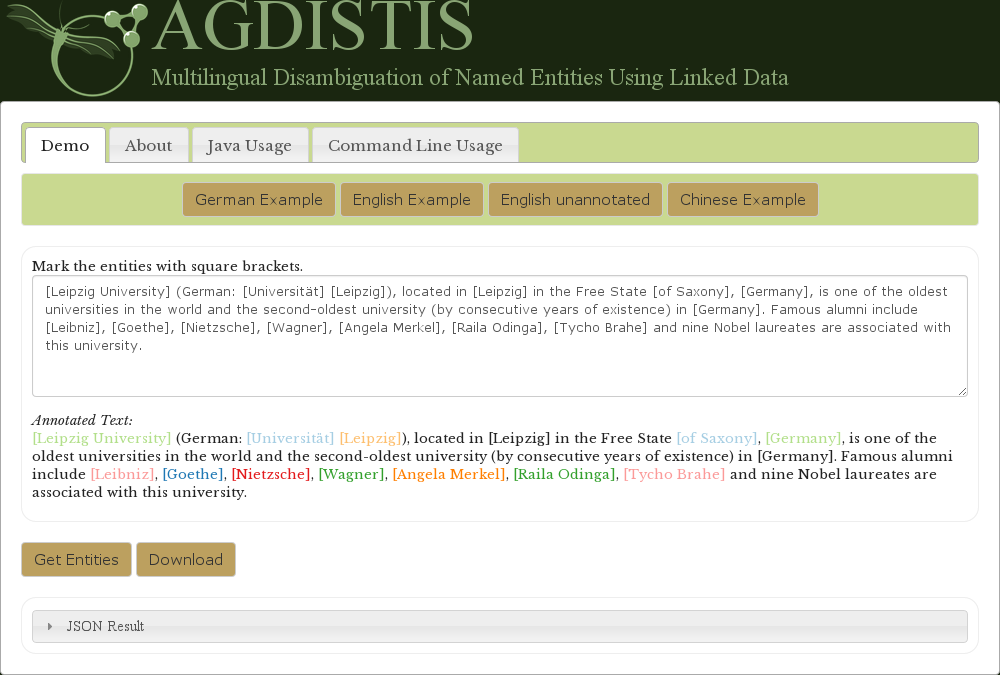
\includegraphics[width=\textwidth]{GUI.png}
\caption{Screenshot of the demo with an English example which is already annotated.}
\label{fig:gui}
\end{figure}

\noindent\textbf{Entity Recognition}
After typing or pasting text into the input field, users can choose between either annotating the entities manually or having the entities detected automatically.
In the first case, the labels of the entities are to be marked by using square brackets (see central panel of Figure~\ref{fig:gui}).
In the case of an automatic annotation, we send the text to the FOX framework, which has been shown to outperform the state of the art in~\cite{FOX}.
%In our current implemen
%Since there is no multilingual NER tool available, an automatic annotation of entities works only for English texts.
We will demonstrate this feature by using both manually pre-annotated text and text without annotations in our examples (see upper bar of Figure~\ref{fig:gui}).
Moreover, we will allow the crowd to enter arbitrary texts that pertain to their domain of interest.

\noindent\textbf{Automatic Language Detection}
Once the user has set which entities are to be disambiguated, the marked-up text is sent to the language detection module based on~\cite{nakatani2010langdetect}.
We chose this library because it is both precise ($>99\%$ precision) and time-efficient.
If the input is detected to belong to one of the languages we support (i.e., German, Chinese, English), then we forward the input to a dedicated AGDISTIS instance for this given language.
In all other cases, an error message is shown to the user, pointing towards the language at hand not being supported.
The main advantage of this approach is that the user does not need to select the language in which the text is explicated manually, thus leading to an improved user experience. 
We will demonstrate this feature by entering text in different languages (German, English, French, Chinese, etc.) and presenting the output of the framework for each of these test cases.

\noindent\textbf{Entity Linking} 
This is the most important step of the whole workflow.
The annotated text is forwarded to the corresponding language-specific deployment of AGDISTIS, of which each relies on a language-specific version of DBpedia 3.9. 
The approach underlying AGDISTIS~\cite{AGDISTIS_ISWC} is language-independent and combines breadth-first search and the well-known HITS algorithm. 
In addition, string similarity measures and label expansion heuristics are used to account for typos and morphological variations in naming.
Moreover, Wikipedia-specific surface forms for resources can be used. 

\noindent\textbf{Output}
Within the demo the annotated text is shown below the input field where disambiguated entities are colored to highlight them. 
While hovering a highlighted entity the disambiguated URI is shown.
We will demonstrate the output of the entity linking by using the examples shown in the upper part of Figure~\ref{fig:gui}. 
The output of the system will be shown both in a HTML version and made available as a download in JSON. 
Moreover, we will allow interested participants to enter their own examples and view the output of the tool.

\subsection{AGDISTIS for expert users}

To support different languages we set up a REST URI for each of the language versions.
%those\footnote{\url{http://139.18.2.164:8080/AGDISTIS_DE}}\footnote{\url{http://139.18.2.164:8080/AGDISTIS_ZH}}\footnote{\url{http://139.18.2.164:8080/AGDISTIS}}.
Each of these endpoints understands two mandatory parameters: (1) \texttt{text} which is an UTF-8 and URL encoded string with entities annotated with XML-tag \texttt{<entity>} and (2) \texttt{type='agdistis'} to disambiguate with the AGDISTIS algorithm.
In the future, several wrappers will be implemented to use different entity linking algorithms for comparison.
Following, a CURL\footnote{\url{http://curl.haxx.se/}} snippet shows how to address the web service, see also \url{http://agdistis.aksw.org}:
\begin{verbatim}
curl --data-urlencode "text='<entity>Barack Obama</entity> arrives 
in <entity>Washington, D.C.</entity>.'" -d type='agdistis' 
{AGDISTIS URL}/AGDISTIS
\end{verbatim}

\section{Evaluation}
\textbf{English and German Evaluation.} AGDISTIS has been evaluated on 8 different datasets from diverse domains such as news, sports or buisiness reports.
For English datasets AGDISTIS is able to outperform the currently best disambiguation framework, TagMe2, on three out of four datasets by up to 29.5\% F-measure. 
Considering the only German dataset available for named entity disambiguation, i.e., \url{news.de}~\cite{N3}, we are able to outperform the only competitor DBpedia Spotlight by 3\% F-measure.


\noindent \textbf{Chinese Evaluation.} We evaluated the Chinese version of AGDISTIS within a question answering setting. 
To this end, we used the multilingual benchmark provided in QALD-4\footnote{\url{http://greententacle.techfak.uni-bielefeld.de/~cunger/qald}}. 
Since the Chinese language is not supported, we extended the QALD-4 benchmark by translating the English questions to Chinese and inserted the named entity links manually.
The accuracies achieved by AGDISTIS for the train and test datasets are 65\% and 70\% respectively. 
%We also performed a fully automatic evaluation by using the Chinese segmentation and named-entity recognition algorithms provided by LTP-Cloud\footnote{\url{http://www.ltp-cloud.com/}}. 
%The accuracies sank to 32\% and 38\%.
%These results indicate the need for better resources for Entity Recognition in Chinese.
\section{Conclusion}
We presented the demo of AGDISTIS for three different languages on three different DBpedia-based knowledge bases.
In future work, we aim to create a single-server multilingual version of the framework that will intrinsically support several languages at the same time.
To this end, we will use a graph merging algorithm to combine the different versions of DBpedia to a single graph.
The disambiguation steps will then be carried out on this unique graph.
%expand different knowledge base and 
%a full dbpedia supported multilingual version



\begin{wrapfigure}[2]{r}{0.20\textwidth}
 \vspace{-8mm}
 
\includegraphics[width=0.20\textwidth]{esf.pdf}
\end{wrapfigure}
\textbf{Acknowledgments} This work has been supported by the ESF and the Free State of Saxony and the FP7 project GeoKnow (GA No. 318159).


\bibliographystyle{plain}
\bibliography{myrefs,aksw,limes,references}


\end{document}

\begin{comment}

\section{How the Chinese version was generated}
\label{sec:chinese}

The key to extend AGDISTIS to support a new language is to provide the needed RDF data for this particular language, especially \texttt{rdf:type} information. 
%However, the latest available Linked Data --- DBpedia 3.9 --- has no such information for Chinese. 
%Therefore, we created triples containing \texttt{rdf:type} as predicate by translating the English ones to Chinese. 
%Specifically, we use inter-language links extracted by DBpedia 
%\footnote{Available from \url{http://wiki.dbpedia.org/Downloads39\#inter-language-links}}, in which a English resource is represented in different other languages. 
%An English-Chinese pair of phrases for each resource is extracted using the following regular expression\footnote{{\it zh} is the language code for Chinese.}:
%\begin{verbatim}
%``$\langle http://dbpedia\backslash.org/resource/(.*)\rangle\backslash s*\langle.*\rangle \backslash s*\langle http://zh.dbpedia.org/resource/(.*)\rangle\backslash s*.$"
%\end{verbatim}
%, resulting a phrase table with 420,047 English-Chinese pairs.

%For each rdf:type triple in the English DBpedia, if the name of the subject appears in the phrase table, it is mapped to Chinese according to the phrase table. In this way, a total of 1,234,783 triples are extrated for Chinese.

%Both the data stored in a Lucene 4.5.1 Index and the phrase table can be found at \url{http://139.18.2.164/rusbeck/}.

%\subsection{Accuracy results of the Chinese version}
%In this section, we will introduce a new Chinese benchmark and the evaluation results.

\subsubsection{Chinese Benchmark}

To evaluate the Chinese version of AGISTIS, a Chinese benchmark is created in the context of question answering because the disambiguation of named entities is a key step to answer a natural language question based on linked data. 

A first try is to adopt the multilingual benchmark provided in QALD-4~\cite{qald4} for question answering. Unfortunately, the Chinese language is not supported. Therefore, we extended the QALD-4 benchmark by translating the English questions to Chinese and annotated the named entity links manually. The links in the given SPARQL queries for the questions are assumed to be the correct links for the English entities, which are adapted to the Chinese links by hand. It results in 200 Chinese questions in the training data and 50 ones in the test data, with an average of 0.9 named entity links per question. The Chinese benchmark is available at \url{https://github.com/wencanluo/DBpediaQA/tree/master/benchmark/qald4}.

\subsubsection{Results}
We first report the disambiguation accuracies by assuming the named entities are given. It allows a fair comparison to other disambiguation algorithms because named entity disambiguation performance is highly depended on named-entity recognition results. The accuracy is measured at a sentence level by assuming a correct disambiguation should recognize and link all the entities in a sentence, which is essential for further steps in question answering. The accuracies for the training and testing are 65\% and 70\% respectively. 

We also performance a fully automatic evaluation by using the Chinese segmentation and named-entity recognition algorithms provided by LTP-Cloud\footnote{\url{http://www.ltp-cloud.com/}}. 
The accuracies are 32\% and 38\%.

architecture, what are the main steps

GOAL is to provide entity linking results to several languages which are show on the website and downloadable as JSON

1 we will present and explain how AGDISTIS works and how multilinguality is achieved

2 Users can try different inputs at the demo station and tell us, what quality they expect and which languages they want

3 finally we will show how the results can be downloaded or seen online and how the annotation of more or less entities changes the behaviour of AGDISTIS

benchmarks will be shown as well and people will be invited to use our for free endpoint for their projects so we can store the use case data and improve our approach similar to the feedback API of spotlight and fox
\end{comment}

\begin{review}
\subsection{Reviewer 1} [DONE by fixing the demo.]
The authors proposed a multilingual disambiguation of named entities system using linked data. The purpose of this paper is to show how AGDISTIS can be used by non-expert based on that system. Through the web site non-expert can get multilingual knowledge which is derived from three different knowledge based such as DBpedia, the German DBpedia and the Chinese DBpedia.

Even though I tried to access the demo site several times, I cannot believe whether this demo site can give the same results which are represented this demo paper as shown figure 1. For instance, when I clicked on the annotate (English only) button I cannot get any text on the result text box. 
\comment: it seems that the "annotate (English only)" works only for session "English unannotated". Thus, it doesn't make sense that all the sessions have such a choice. 

Also sometimes I have got proxy error. Thus I cannot check this service easily.

In addition, the detail explanation of AGDISTIS will be presented on this conference. Therefore I am still doubtful about the purpose of this demo paper.

Therefore, I would like to decide to reject this paper since that contribution. However, if the authors can update the demo system then I will check this system again and I am going to make a final decision at that time.
Before submitting of the final version, please check the order of referred papers. [done]

\subsection{Reviewer 2}
The submission demonstrates AGDISTIS, a system for disambiguating named entities in multilingual texts against a generic RDF knowledge base. While details of AGDISTIS are presented in an accepted ISWC research paper, the proposed demo would allow attendees of the Poster and Demo session to interact with the real system through the submission of both example and arbitrary multilingual texts (English, German, Chinese).

Overall, the paper is well written and the demonstration is clearly described (although I wasn't able to try the online version - I fear I made it crash...). In particular, the demonstrator capability of accepting arbitrary text and invoking also DBpedia Spotlight for comparison would allow attendees to better appreciate the contribution presented at the research track, giving them the possibility to analyze and contrast AGDISTIS performances on borderline cases. For that reason, I reccommend the submission to be accepted as a demo.

As minor notes, it would be nice if the authors could specify whether and how the AGDISTIS software will be made available (source code seems to be available under MIT license) and, if it is the case, how complex would be for a user to reuse AGDISTIS in his own application / research work (e.g., how complex it is to apply it to a specific RDF knowledge base). Moreover, it would be great if the demonstrator could expose some detail on the internal functioning of AGDISTIS, e.g., to help attendees to better understand why and how an entity was selected for linking rather than another candidate.

Typos and other minor issues:
- pg. 2: ...either annotating the entities manually *OR* having the entities detected automatically -> add OR [fixed]
- pg. 2: ...the labels of the entities are to *BE* marked... -> add BE [fixed]
- pg. 3: ...belong to one of the language*S*... -> add S [fixed]
- pg. 3: ...is language-independent and *IS* combines... -> remove IS [fixed]
- pg. 3: in the CURL snippet I suggest a more meaningful example than "University of Leipzig in Barack Obama" [fixed]
- pg. 4: I suggest checing capitalization of words in the references section [fixed]

\subsection{Reviewer 3}
The paper presents AGDISTIS, a system for multilingual named entity resolution and linking.
The authors provide a link to a Web interface that make it clear the subject of the demonstration.
Additionally, the authors provide a detailed documentation about how to use the system by means of HTTP REST API.
The technical quality and the readability of the paper are good.

However, some points remain unclear:
* to what extent the system is knowledge-base-agnostic?
* how is it possible to extend the set of languages that the system is able to deal with?

\end{review}
